\documentclass[12pt,oneside]{book}
\usepackage{times,mathptmx}
\usepackage[pdftex]{graphicx}
\usepackage{calc}
\usepackage{tabularx,ragged2e,booktabs,caption,subcaption}
\usepackage{array}
\newcolumntype{L}[1]{>{\raggedright\let\newline\\\arraybackslash\hspace{0pt}}m{#1}}
\newcolumntype{C}[1]{>{\centering\let\newline\\\arraybackslash\hspace{0pt}}m{#1}}
\newcolumntype{R}[1]{>{\raggedleft\let\newline\\\arraybackslash\hspace{0pt}}m{#1}}
\usepackage{multirow}
\usepackage{tocloft}
\usepackage{xcolor}
\usepackage{color,soul}
\usepackage{amsmath}
\definecolor{linknavy}{rgb}{0,0,0.50196}
\definecolor{linkred}{rgb}{1,0,0}
\definecolor{linkblue}{rgb}{0,0,1}
\usepackage{float}
\usepackage{graphpap}
\usepackage{rotating}
\usepackage{graphicx}
\usepackage{geometry}
\usepackage{relsize}
\usepackage{ltablex}
\usepackage{longtable}
\usepackage{lscape}
\usepackage{amssymb}
\usepackage{makeidx} % Create index at end of document
\usepackage[nottoc,notlof,notlot]{tocbibind} % Put the bibliography and index in the ToC
\usepackage{lastpage} % Automatic last page number reference.
\usepackage[T1]{fontenc}
\usepackage{enumerate}
\usepackage{upquote}
\usepackage{moreverb}
\usepackage{xfrac}
\usepackage{cite}
\usepackage{tikz}
% \usepackage{subfig}
% \usepackage{caption}
\usepackage[toc,page]{appendix}
\usepackage{notoccite}
\usepackage{colortbl}
\usepackage{titlesec}
\titleformat{\chapter}[hang] 
{\normalfont\huge\bfseries}{\chaptertitlename\ \thechapter}{1em}{} 
\titlespacing*{\chapter}{0pt}{-30pt}{20pt}

\newcommand{\nopart}{\expandafter\def\csname Parent-1\endcsname{}} % To fix table of contents in pdf.

\usepackage{siunitx}
\sisetup{
    detect-all = true,
    input-decimal-markers = {.},
    input-ignore = {,},
    inter-unit-product = \ensuremath{{}\cdot{}},
    multi-part-units = repeat,
    number-unit-product = \text{~},
    per-mode = fraction,
    separate-uncertainty = true,
}

\usepackage{listings}
\usepackage{textcomp}
\definecolor{lbcolor}{rgb}{0.96,0.96,0.96}

\usepackage[pdftex,
        colorlinks=true,
        urlcolor=linkblue,     % \href{...}{...} external (URL)
        citecolor=linkred,     % citation number colors
        linkcolor=linknavy,    % \ref{...} and \pageref{...}
        pdfproducer={pdflatex},
        pdfpagemode=UseNone,
        bookmarksopen=true,
        plainpages=false,
        verbose]{hyperref}

\setlength{\textwidth}{6.5in}
\setlength{\textheight}{9.0in}
\setlength{\topmargin}{0.in}
\setlength{\headheight}{0.pt}
\setlength{\headsep}{0.in}
\setlength{\parindent}{0.0in}
\setlength{\itemindent}{0.25in}
\setlength{\oddsidemargin}{0.0in}
\setlength{\evensidemargin}{0.0in}
% \setlength{\leftmargini}{\parindent} % Controls the indenting of the "bullets" in a list
\setlength{\cftsecnumwidth}{0.45in}
\setlength{\cftsubsecnumwidth}{0.5in}
\setlength{\cftfignumwidth}{0.45in}
\setlength{\cfttabnumwidth}{0.45in}
\setlength{\parskip}{1em}

\newcommand{\titlesigs}
{
\large
\flushright{UL Firefighter Safety Research Institute\\
{\em Stephen Kerber, Director} \\
\hspace{1in} \\
}
}

\newcommand{\headerB}[1]{
\flushleft{
\fontsize{28}{33.6}\selectfont
\bf{#1}
}
}

\newcommand{\headerC}[1]{
\vspace{.5in}
\flushright{\fontsize{14}{16.8}\selectfont
#1}
}

% \newcolumntype{L}{>{\centering\arraybackslash}m{4cm}}

\floatstyle{boxed}
\newfloat{notebox}{H}{lon}
\newfloat{warning}{H}{low}

\newenvironment{conditions}
  {\par\vspace{\abovedisplayskip}\noindent\begin{tabular}{>{$}l<{$} @{${}={}$} l}}
  {\end{tabular}\par\vspace{\belowdisplayskip}}


%rename chapter headings
\renewcommand{\chaptername}{}
\renewcommand{\bibname}{References}

\usepackage{fancyhdr}
\pagestyle{fancy}
\lhead{}
\rhead{}
\chead{}
\renewcommand{\headrulewidth}{0pt}

\usepackage{draftwatermark}
\SetWatermarkText{DRAFT}
\SetWatermarkScale{1}

\begin{document}
\pagenumbering{gobble}
\bibliographystyle{unsrt}
	
\begin{minipage}[t][9in][s]{6.25in}

\headerB{
Impact of Fire Attack Utilizing \\
Interior and Exterior Streams on \\
Firefighter Safety and Occupant Survival: Howard Room Experiments \\
}

\normalsize

\headerC{
	{ \flushleft{
	Keith Stakes \\
	Robin Zevotek \\
	\vspace{0.2in}
	UL Firefighter Safety Research Institute \\
	Columbia, MD 20145 \\
	\vspace*{2\baselineskip}

	} 

	\vfill

	\flushright{

	
\includegraphics[width=2.0in]{Figures/General/FSRI_GraphicShield.pdf} \\ [.3in]

	}
	}
	}

\end{minipage}

\newpage
\hspace{5in}
\newpage

\frontmatter

\begin{minipage}[t][9in][s]{6.25in}
\pagenumbering{gobble}


\headerB{
Impact of Fire Attack Utilizing \\
Interior and Exterior Streams on\\ 
Firefighter Safety and Occupant \\
Survival: Air Entrainment\\
}

\headerC{
\flushleft{
Keith Stakes \\
Robin Zevotek \\
\vspace{0.2in}
{UL Firefighter Safety Research Institute \\
Columbia, MD 21045 \\}}

\flushleft{\today \\}
}


\vfill

\flushright{
\includegraphics[width=2in]{Figures/General/FSRI_GraphicShield.pdf}}

\titlesigs

\end{minipage}

\frontmatter

\chapter{Test Set Up}

\section{Structures}

These room fire experiments were conducted in two identical structures that were constructed on the grounds of the Howard County (MD) Public Safety Training Facility. The 237~sq.~ft. text fixture included a bedroom and adjoining hallway. The dimensions of the structure were identical to that of the master bedroom (bedroom 1) and the hallway found within the structures utilized during the full-scale fire experiments conducted in Northbrook, IL at UL's Large Fire Lab. The interior of the test fixture had 8~ft. ceilings and the room was separated from the hallway with an open doorway of common size (30~in. by 80~in.). There was a hollow core, outswinging, door located at the end of the hallway, also of common size (30~in. by 80~in.). The floor plan of the test fixtures used for these experiments can be seen in Figure~\ref{fig:floorplan}.

\begin{figure}[H]
\centering
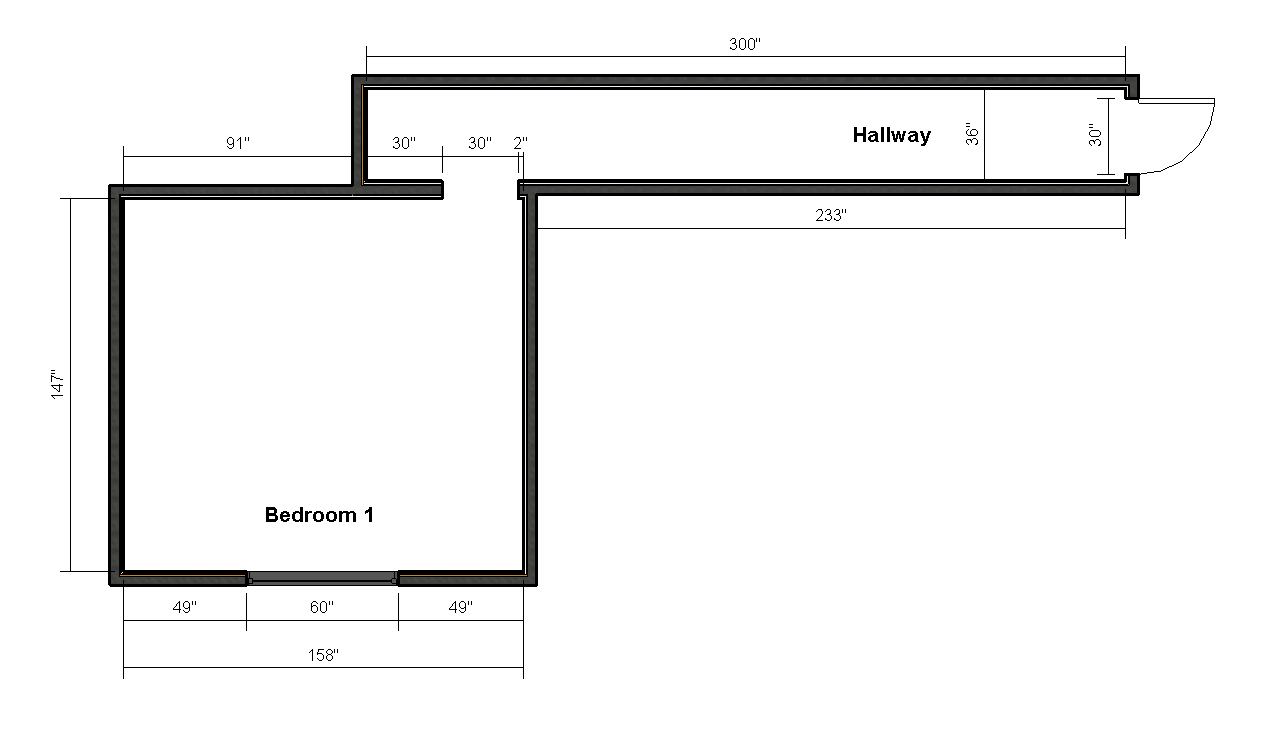
\includegraphics[width=\textwidth]{Figures/Structures/floorplan.png}
\caption{Floor Plan}
\label{fig:floorplan}
\end{figure}

Since these room fire experiments were intended to examine room and contents fires, and not structure fires, the walls of the fire room (Bedroom 1) and hallway were lined with two layers of gypsum board: a surface layer of 1/2~in. board and a base layer, also of 1/2~in. board. The exterior wall outside of the bedroom 1 window was covered with cement board to limit exterior fire spread. The exterior of bedroom 1 can be seen in Figure~\ref{fig:bedroomext}, and the interior hallway with finished drywall can be seen in Figure~\ref{fig:inthallway}.

\begin{figure}[H]
\centering
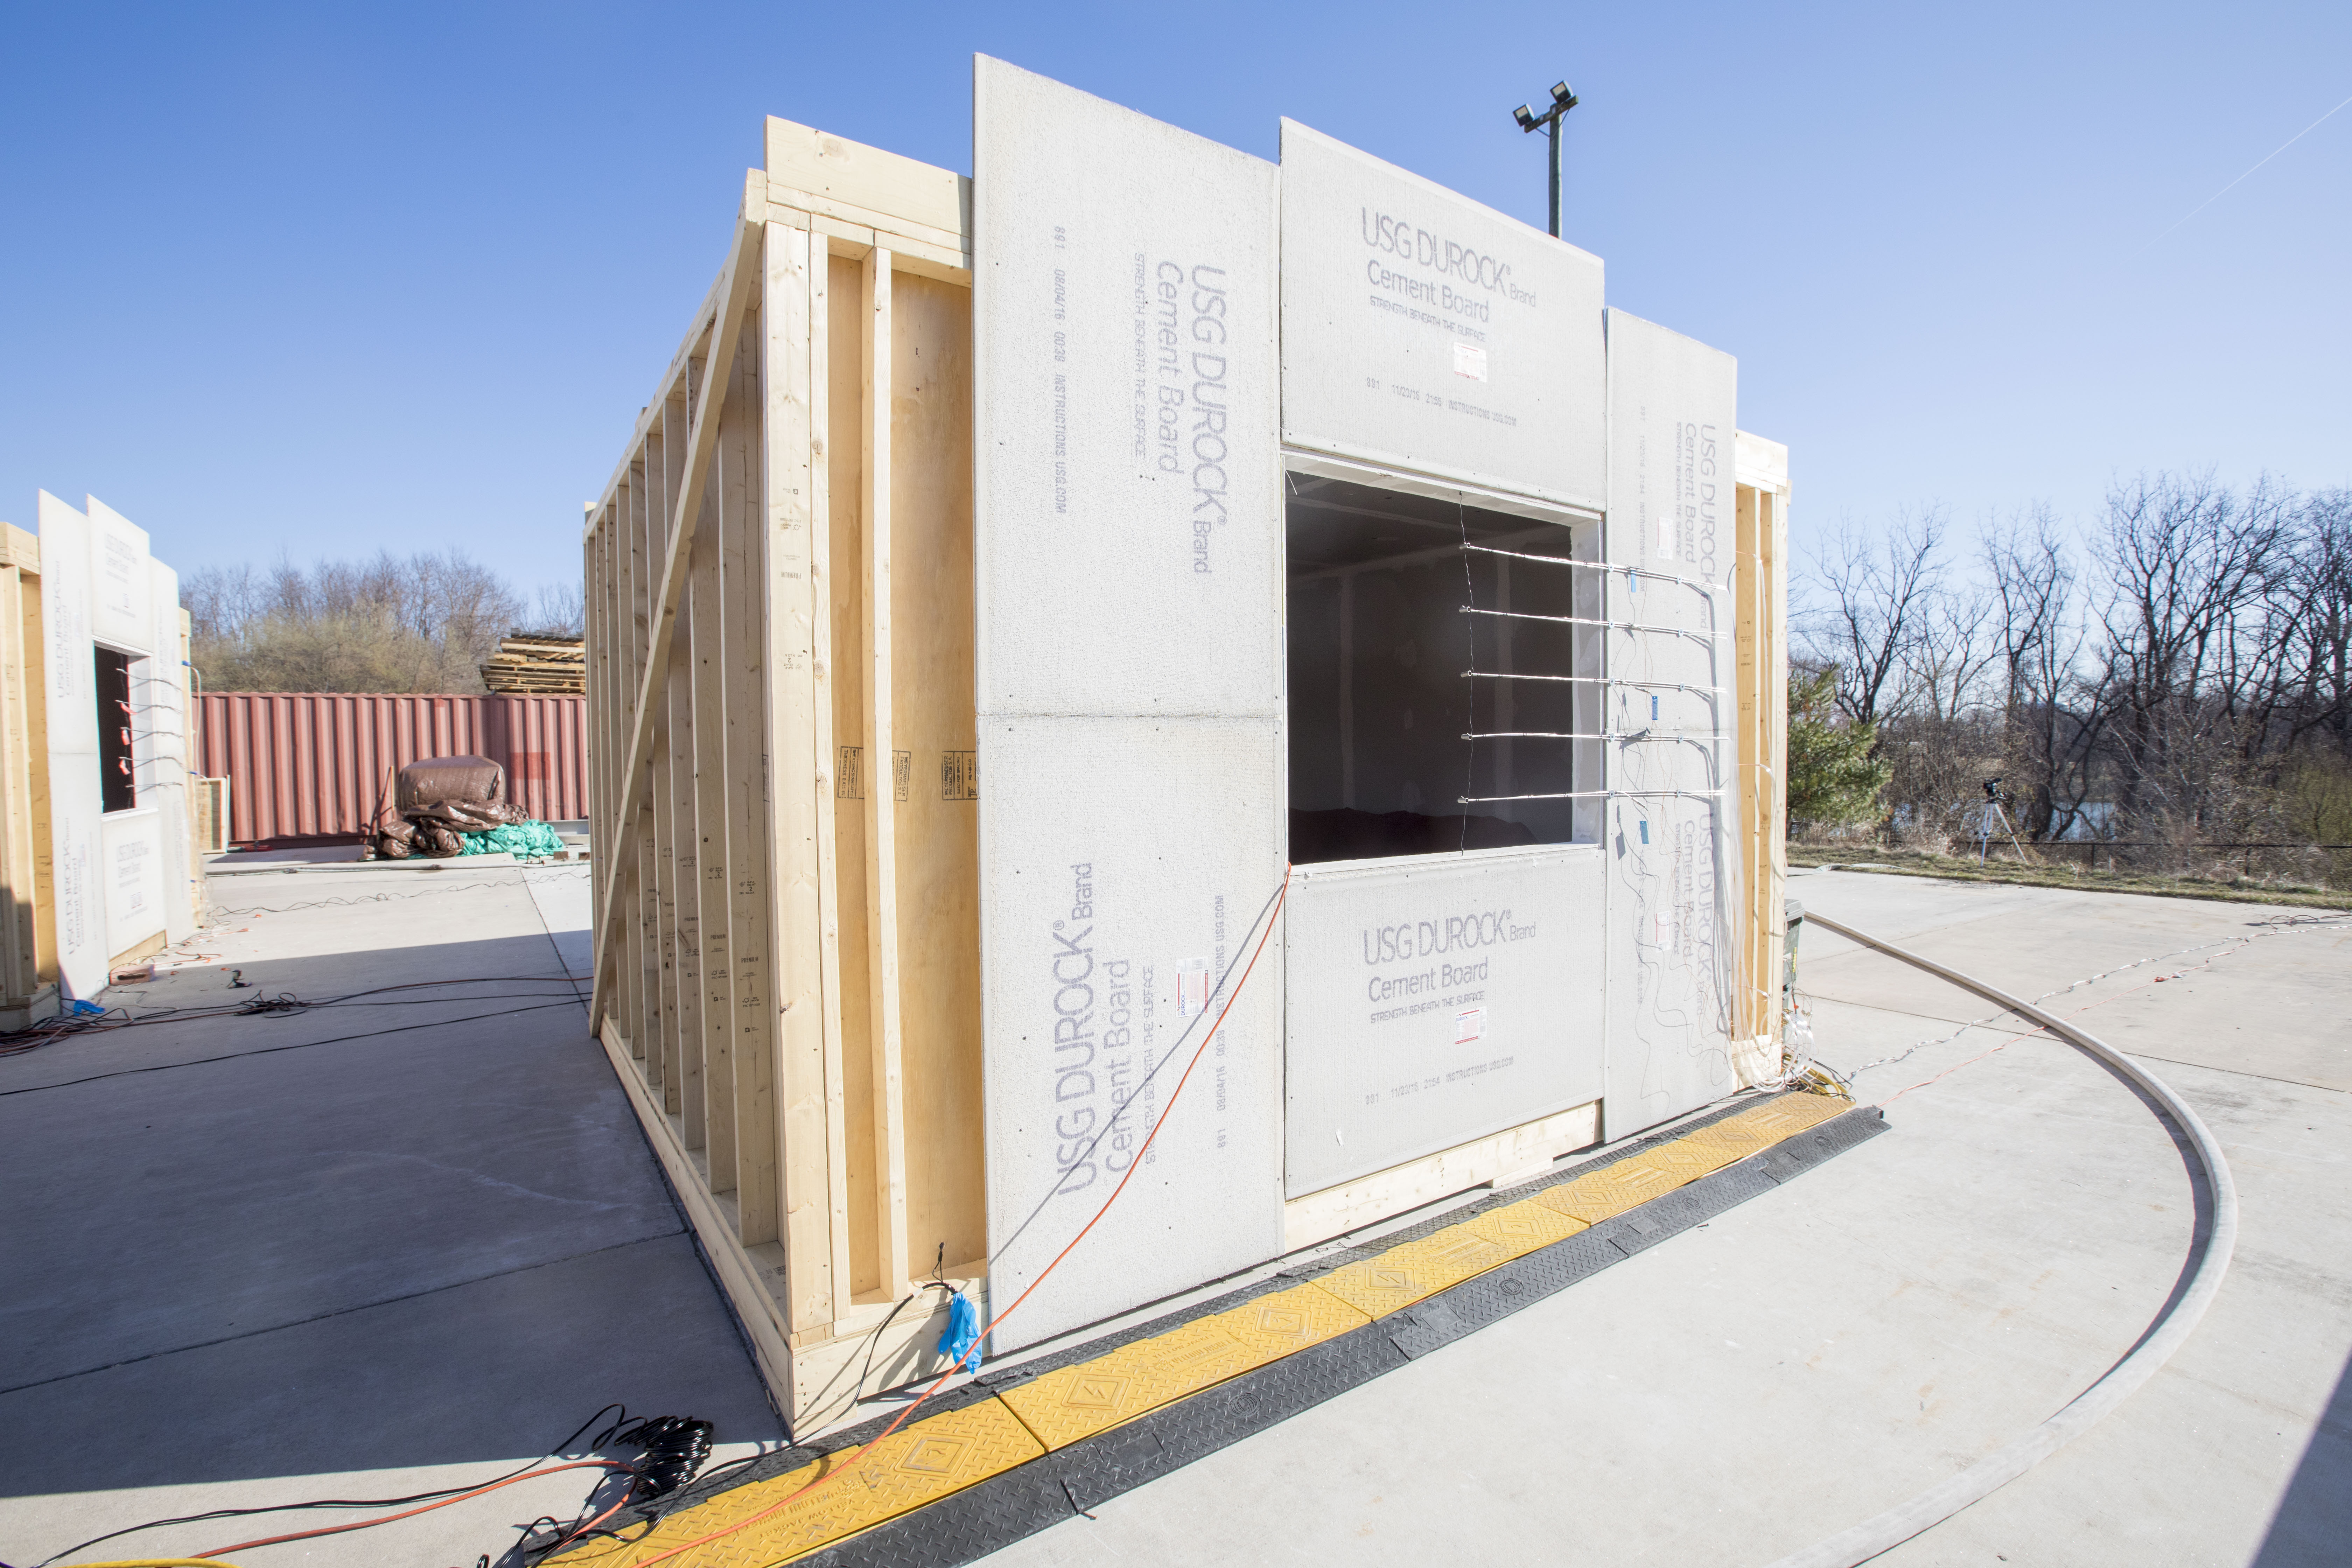
\includegraphics[width=\textwidth]{Figures/Structures/bedroomext.png}
\caption{Exterior of Bedroom 1}
\label{fig:bedroomext}
\end{figure}

\begin{figure}[H]
\centering
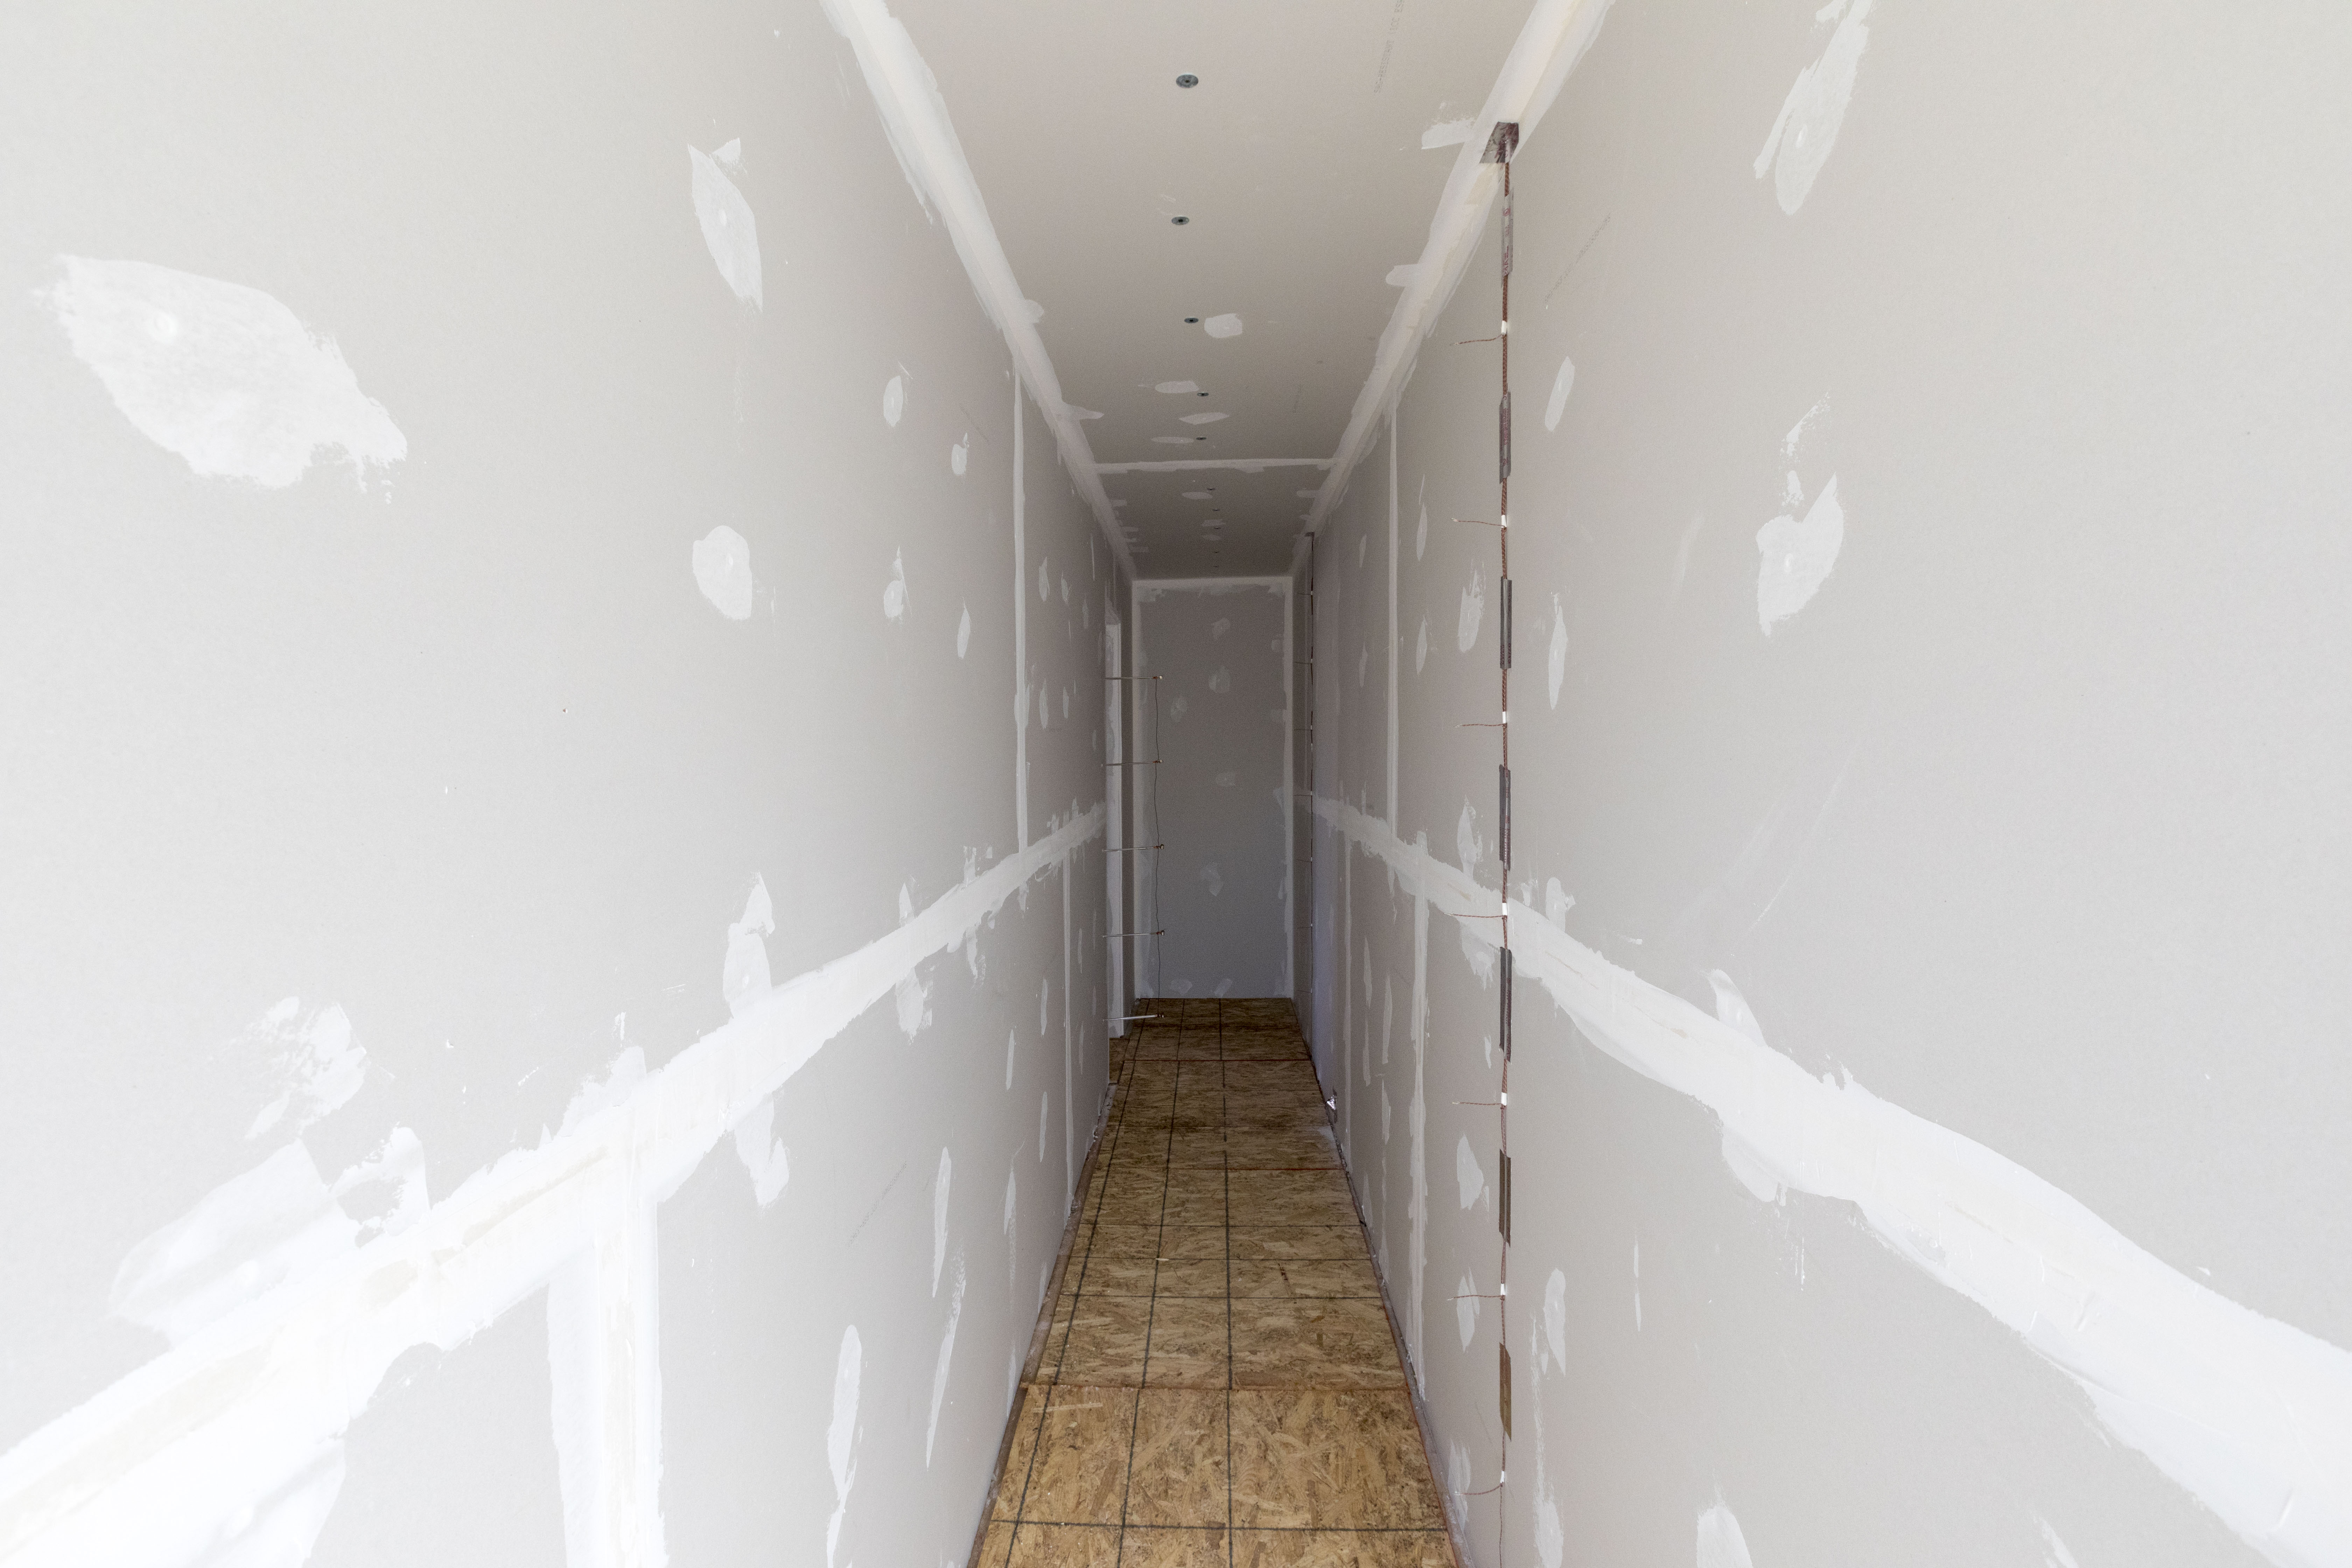
\includegraphics[width=\textwidth]{Figures/Structures/inthallway.png}
\caption{Interior Hallway}
\label{fig:inthallway}
\end{figure}

\paragraph{Air Leakage in the Structure}

The leakage of the structure was determined through the use of a blower door test in accordance with ANSI E1872. A retotec model 5101 blower door was used in accordance with the user manual~\cite{RetroTecManual}.

The standard for leakage of a structure is determined by the IECC. In 2009 the leakage for all climate zones could not exceed 7 air changes per hour. In the 2012 version of the standard the requirement was increased to less than or equal 5 air changes per hour for climate zones 1 and 2 and less than 3 air changes per hour for climate zones 3 $-$ 8.  The structure had a leakage rate of \hl{25 air changes per hour} making it more consistent with leakage found in homes constructed prior to the 2009 IECC. 

Another measure of the leakage, Equivalent Leakage Area (ELA) was also calculated through the use of the blower door. This measurement takes into account all the leakage in a structure, as a flow, and calculates an opening size required to permit that flow. The structures used had an equivalent leakage area of \hl{1.2 $ft^2$}. This is equivalent to having a \hl{15"} diameter hole in the structure. In reality this area is distributed throughout all the smaller openings like those found around windows; however, this calculation allows for the visualization of the size of opening required to provide the leakage rate found in the test fixture utilized. 

\section{Furnishings}

Furniture was acquired for the experiments such that each room of furniture was the same from experiment to experiment. Descriptions and dimensions for all of the furniture used are in Table~\ref{FurnitureTable}. Images of each piece of furniture can be seen in Figure~\ref{fig:FurnitureImages}.

\renewcommand{\arraystretch}{1.5}
\begin{table}[H]
	\centering
	\caption{Furniture Dimensions and Weight}
		\begin{tabular}[c]{|c|c|c|c|}
			\hline
			\textbf{Item} & \textbf{Length (in.)} & \textbf{Width (in.)} & \textbf{Height (in.)} \\ \hline \hline
			Sofa & 89 & 39 & 40 \\ \hline
			Mattress & 75 & 54 & 7.5 \\ \hline
			Box Spring & 75 & 54 & 12 \\ \hline
		\end{tabular}
	\label{FurnitureTable}
\end{table}

% \begin{figure}
% 	\centering
% 	\begin{tabular}[c]{c c}
% 		\subfloat[Sofa]{\includegraphics[width=6cm]{Figures/Furniture/sofa.jpg}} &
% 		\subfloat[Mattress \& Boxspring]{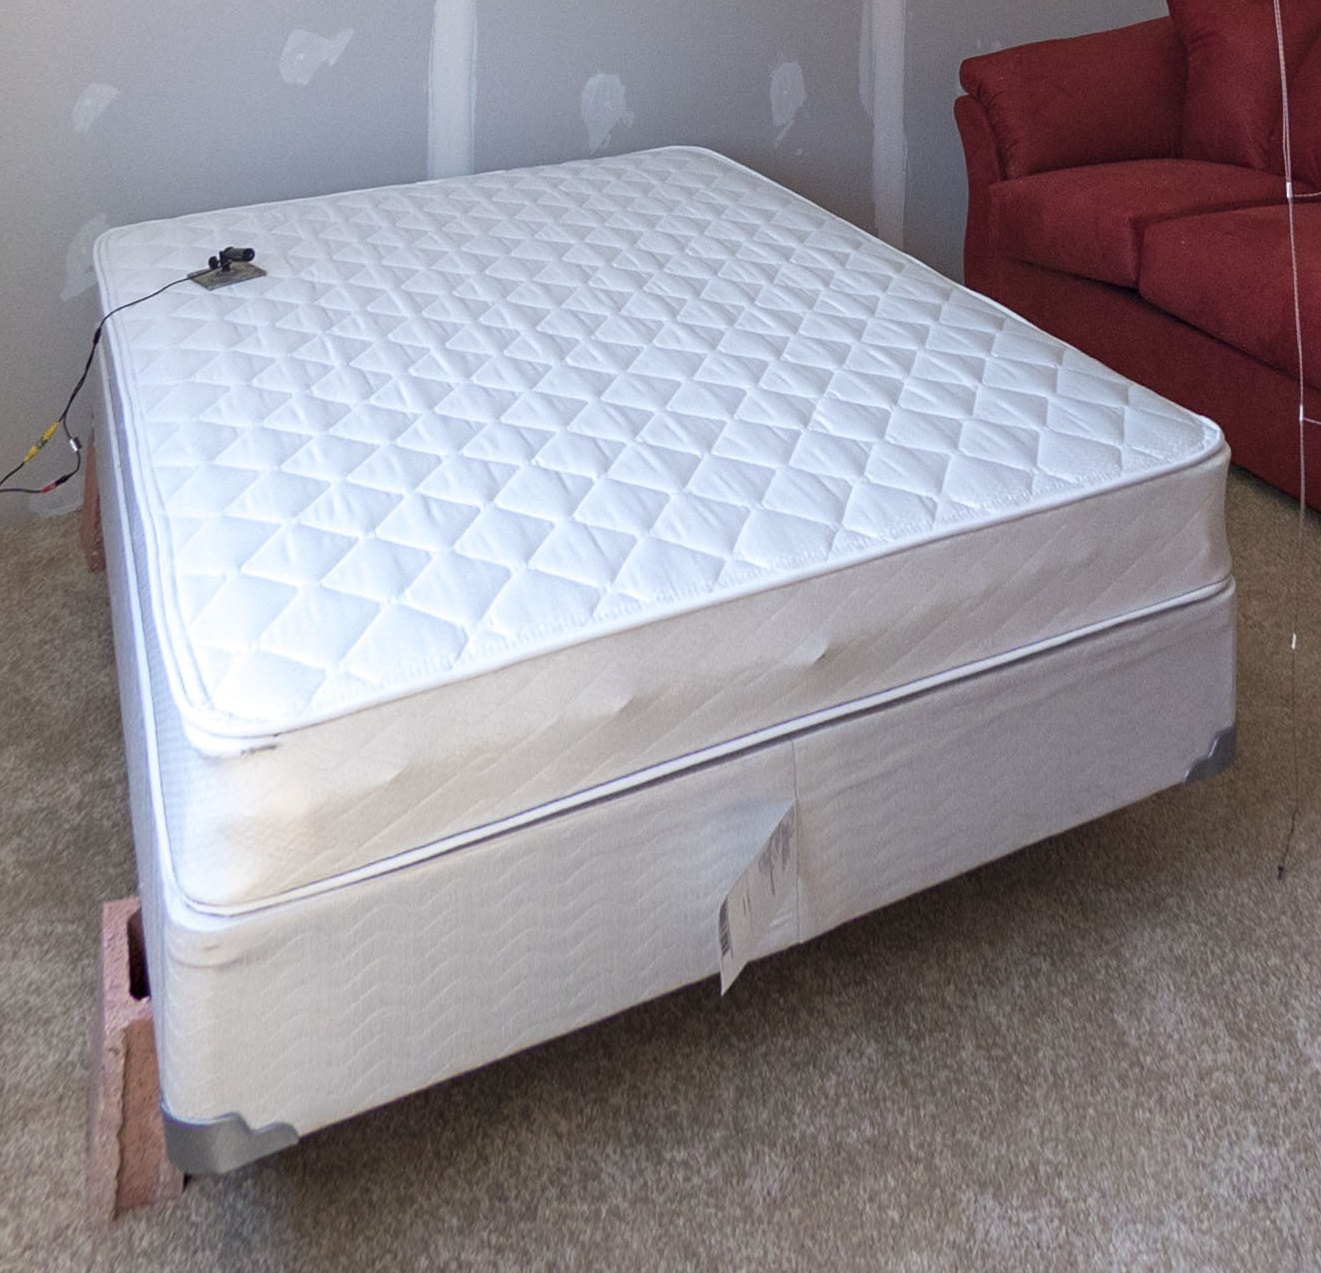
\includegraphics[width=6cm]{Figures/Furniture/bed.jpg}} \\
% 	\end{tabular}
% 	\caption{Furniture Images}
% 	\label{fig:FurnitureImages}
% \end{figure}

\begin{figure}[ht]
  \centering
  \begin{subfigure}[Sofa]{0.5\linewidth}
    \centering\includegraphics[width=6cm]{Figures/Furniture/sofa.jpg}
    \caption{\label{fig:Sofa}}
  \end{subfigure}%
  \begin{subfigure}[Bed]{0.5\linewidth}
    \centering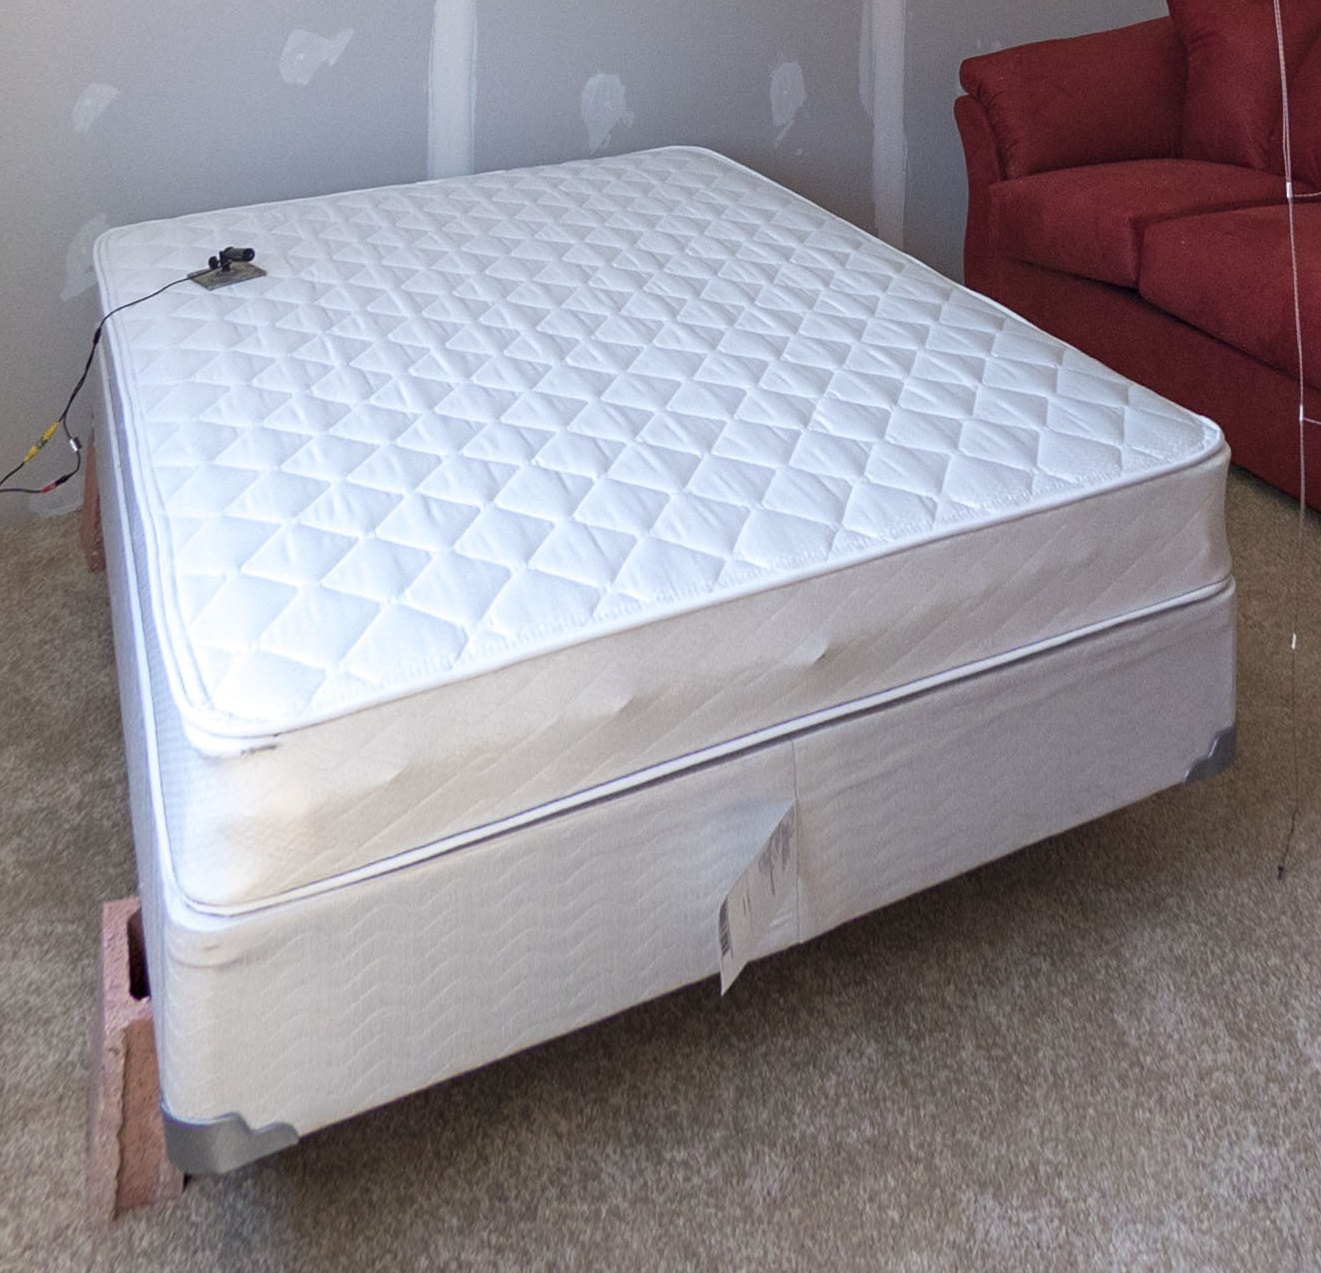
\includegraphics[width=6cm]{Figures/Furniture/bed.jpg}
    \caption{\label{fig:Bed}}
  \end{subfigure}
  \caption{Picture~\subref{fig:Sofa} shows the sofa and Picture~\subref{fig:Bed} shows the mattress and boxspring used as furnishings for these experiments.}
  \label{fig:FurnitureImages}
\end{figure}

For Experiment 1, the bedroom in the structure was furnished with two full-size sofas. The floor was covered with 7/16~in. oriented strand board (OSB). For Experiments 2 through 6, the bedroom in the structure was furnished with a mattress \& boxspring (full size) and two full-size sofas. The floor was covered with 7/16~in. OSB, polyurethane foam padding, and polyester carpet. Figures~\ref{fig:Exp1Furniture} and~\ref{fig:Exp2to6Furniture} show the bedroom furniture setup for all of the experiments conducted.

\begin{figure}[H]
	\centering
	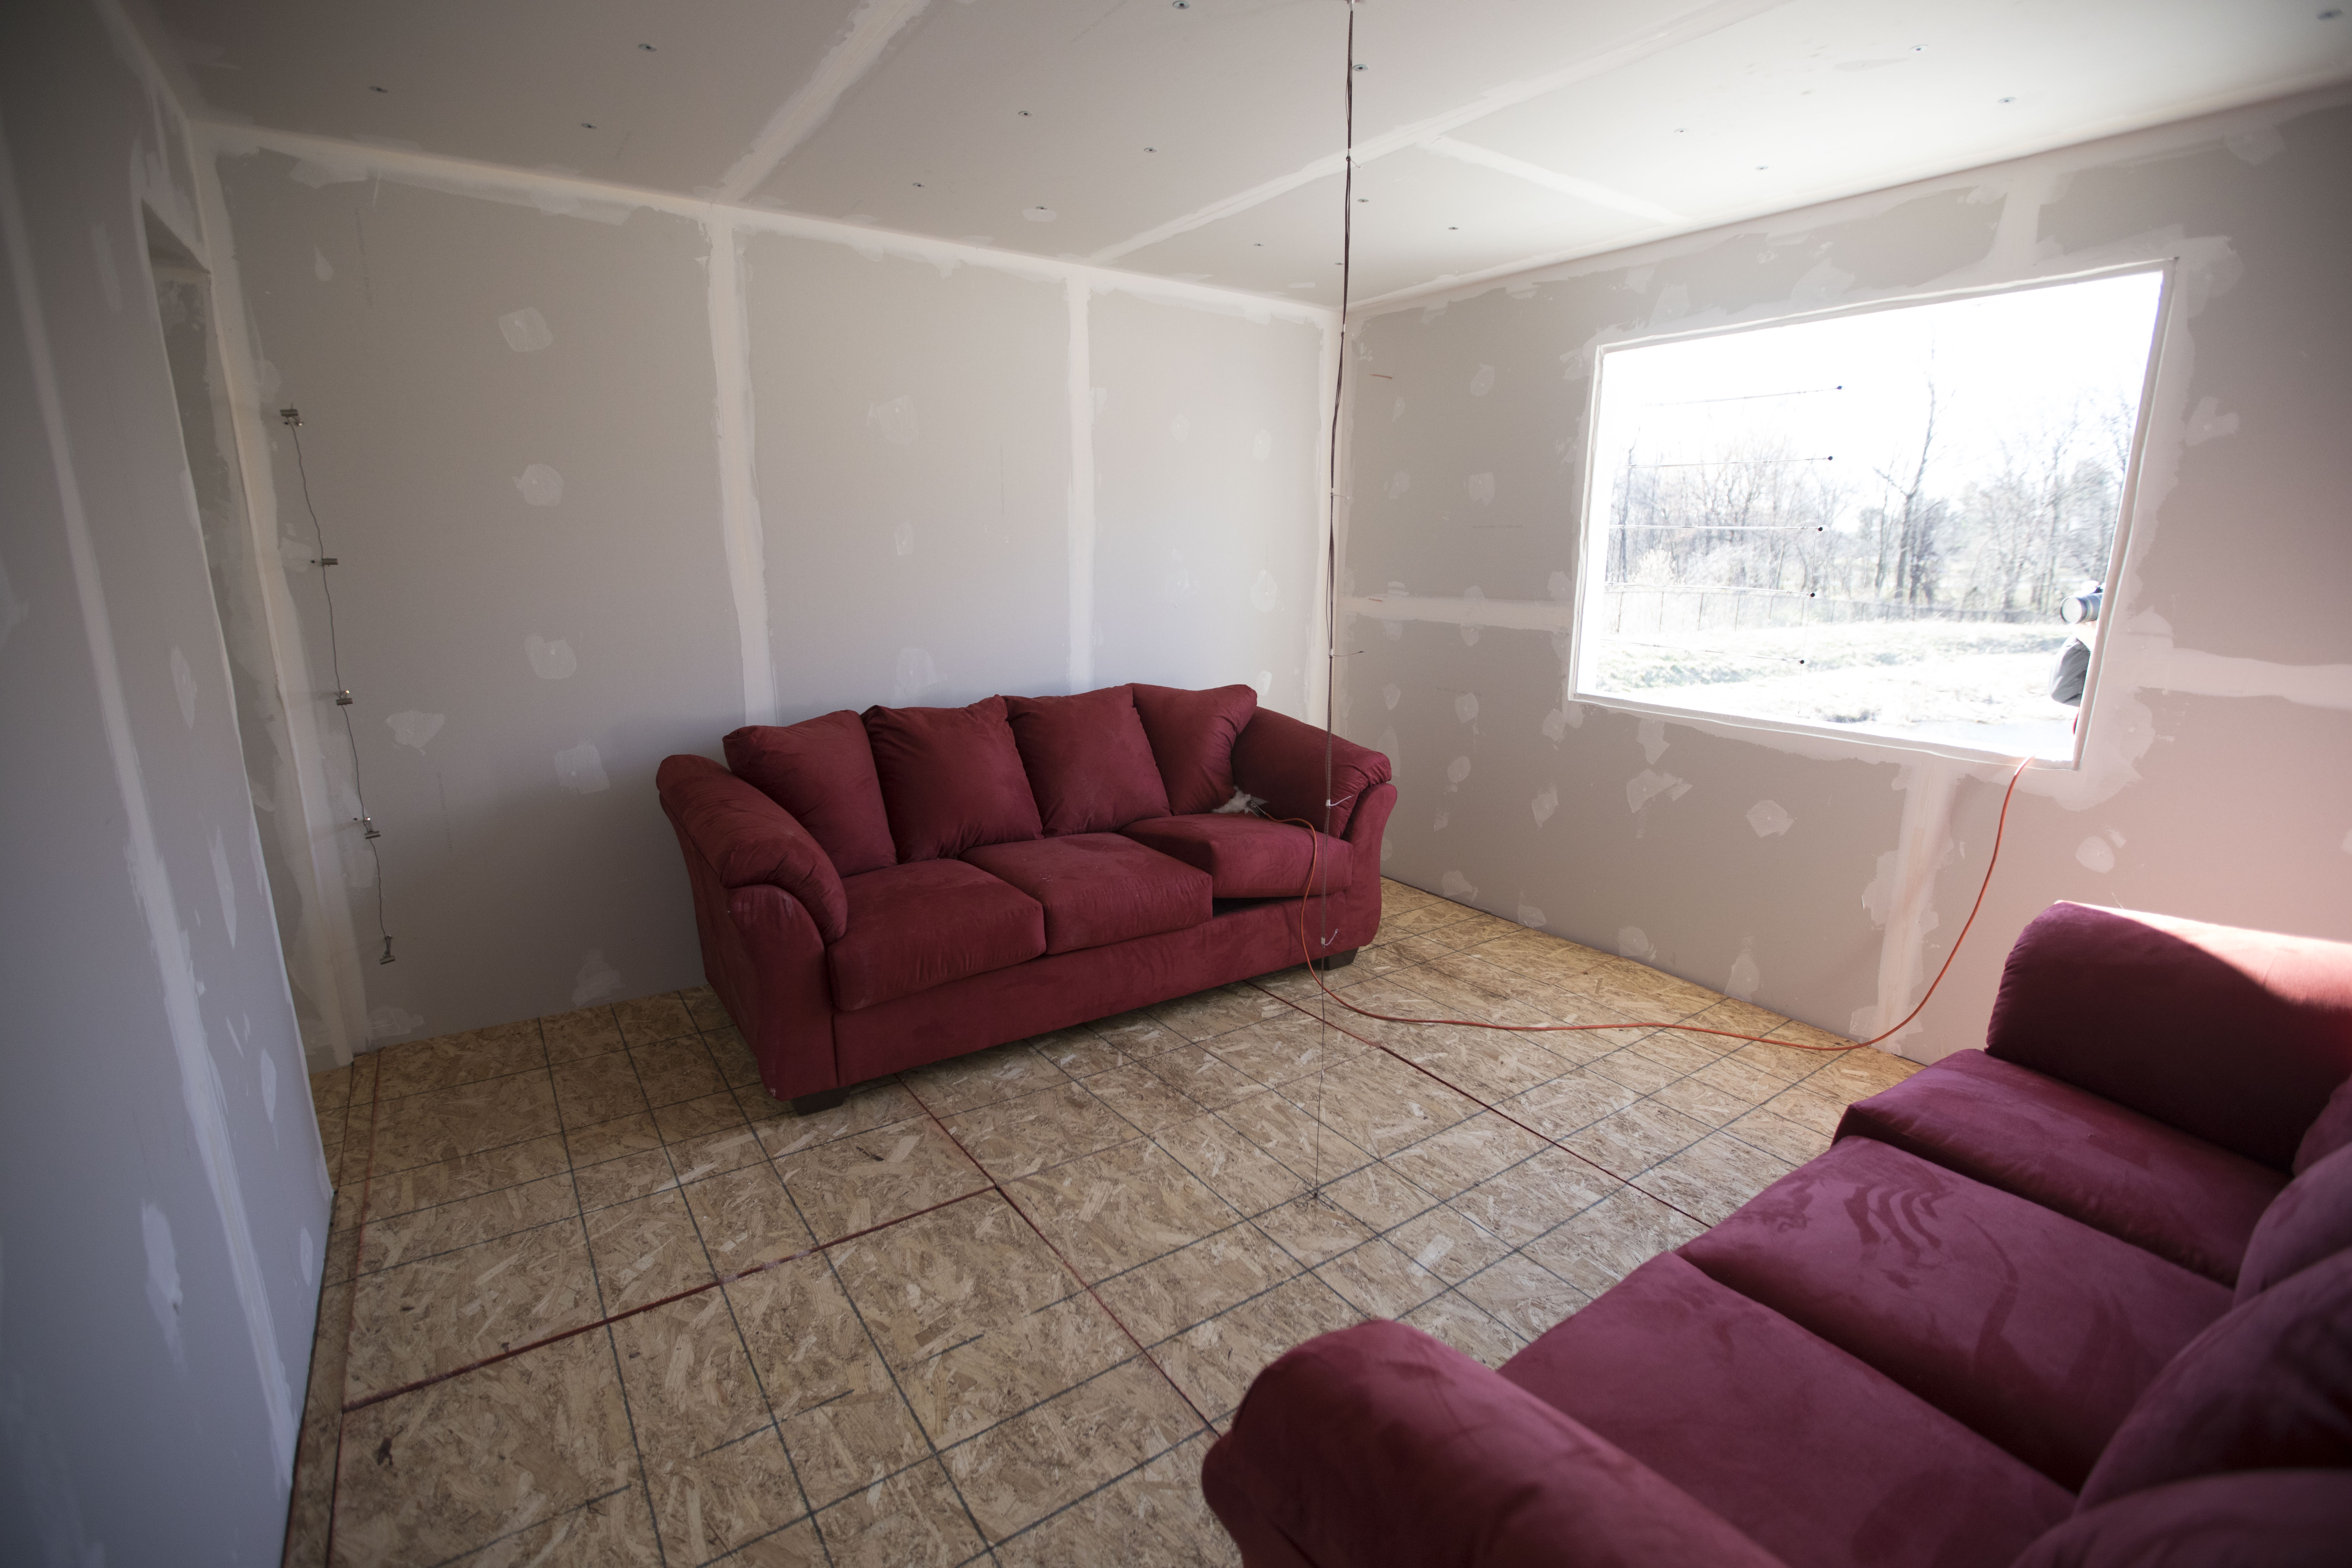
\includegraphics[width=\textwidth]{Figures/Furniture/Exp1Furniture.jpg}
	\caption{Experiment 1 Furniture Layout}
	\label{fig:Exp1Furniture}
\end{figure}

\begin{figure}[H]
	\centering
	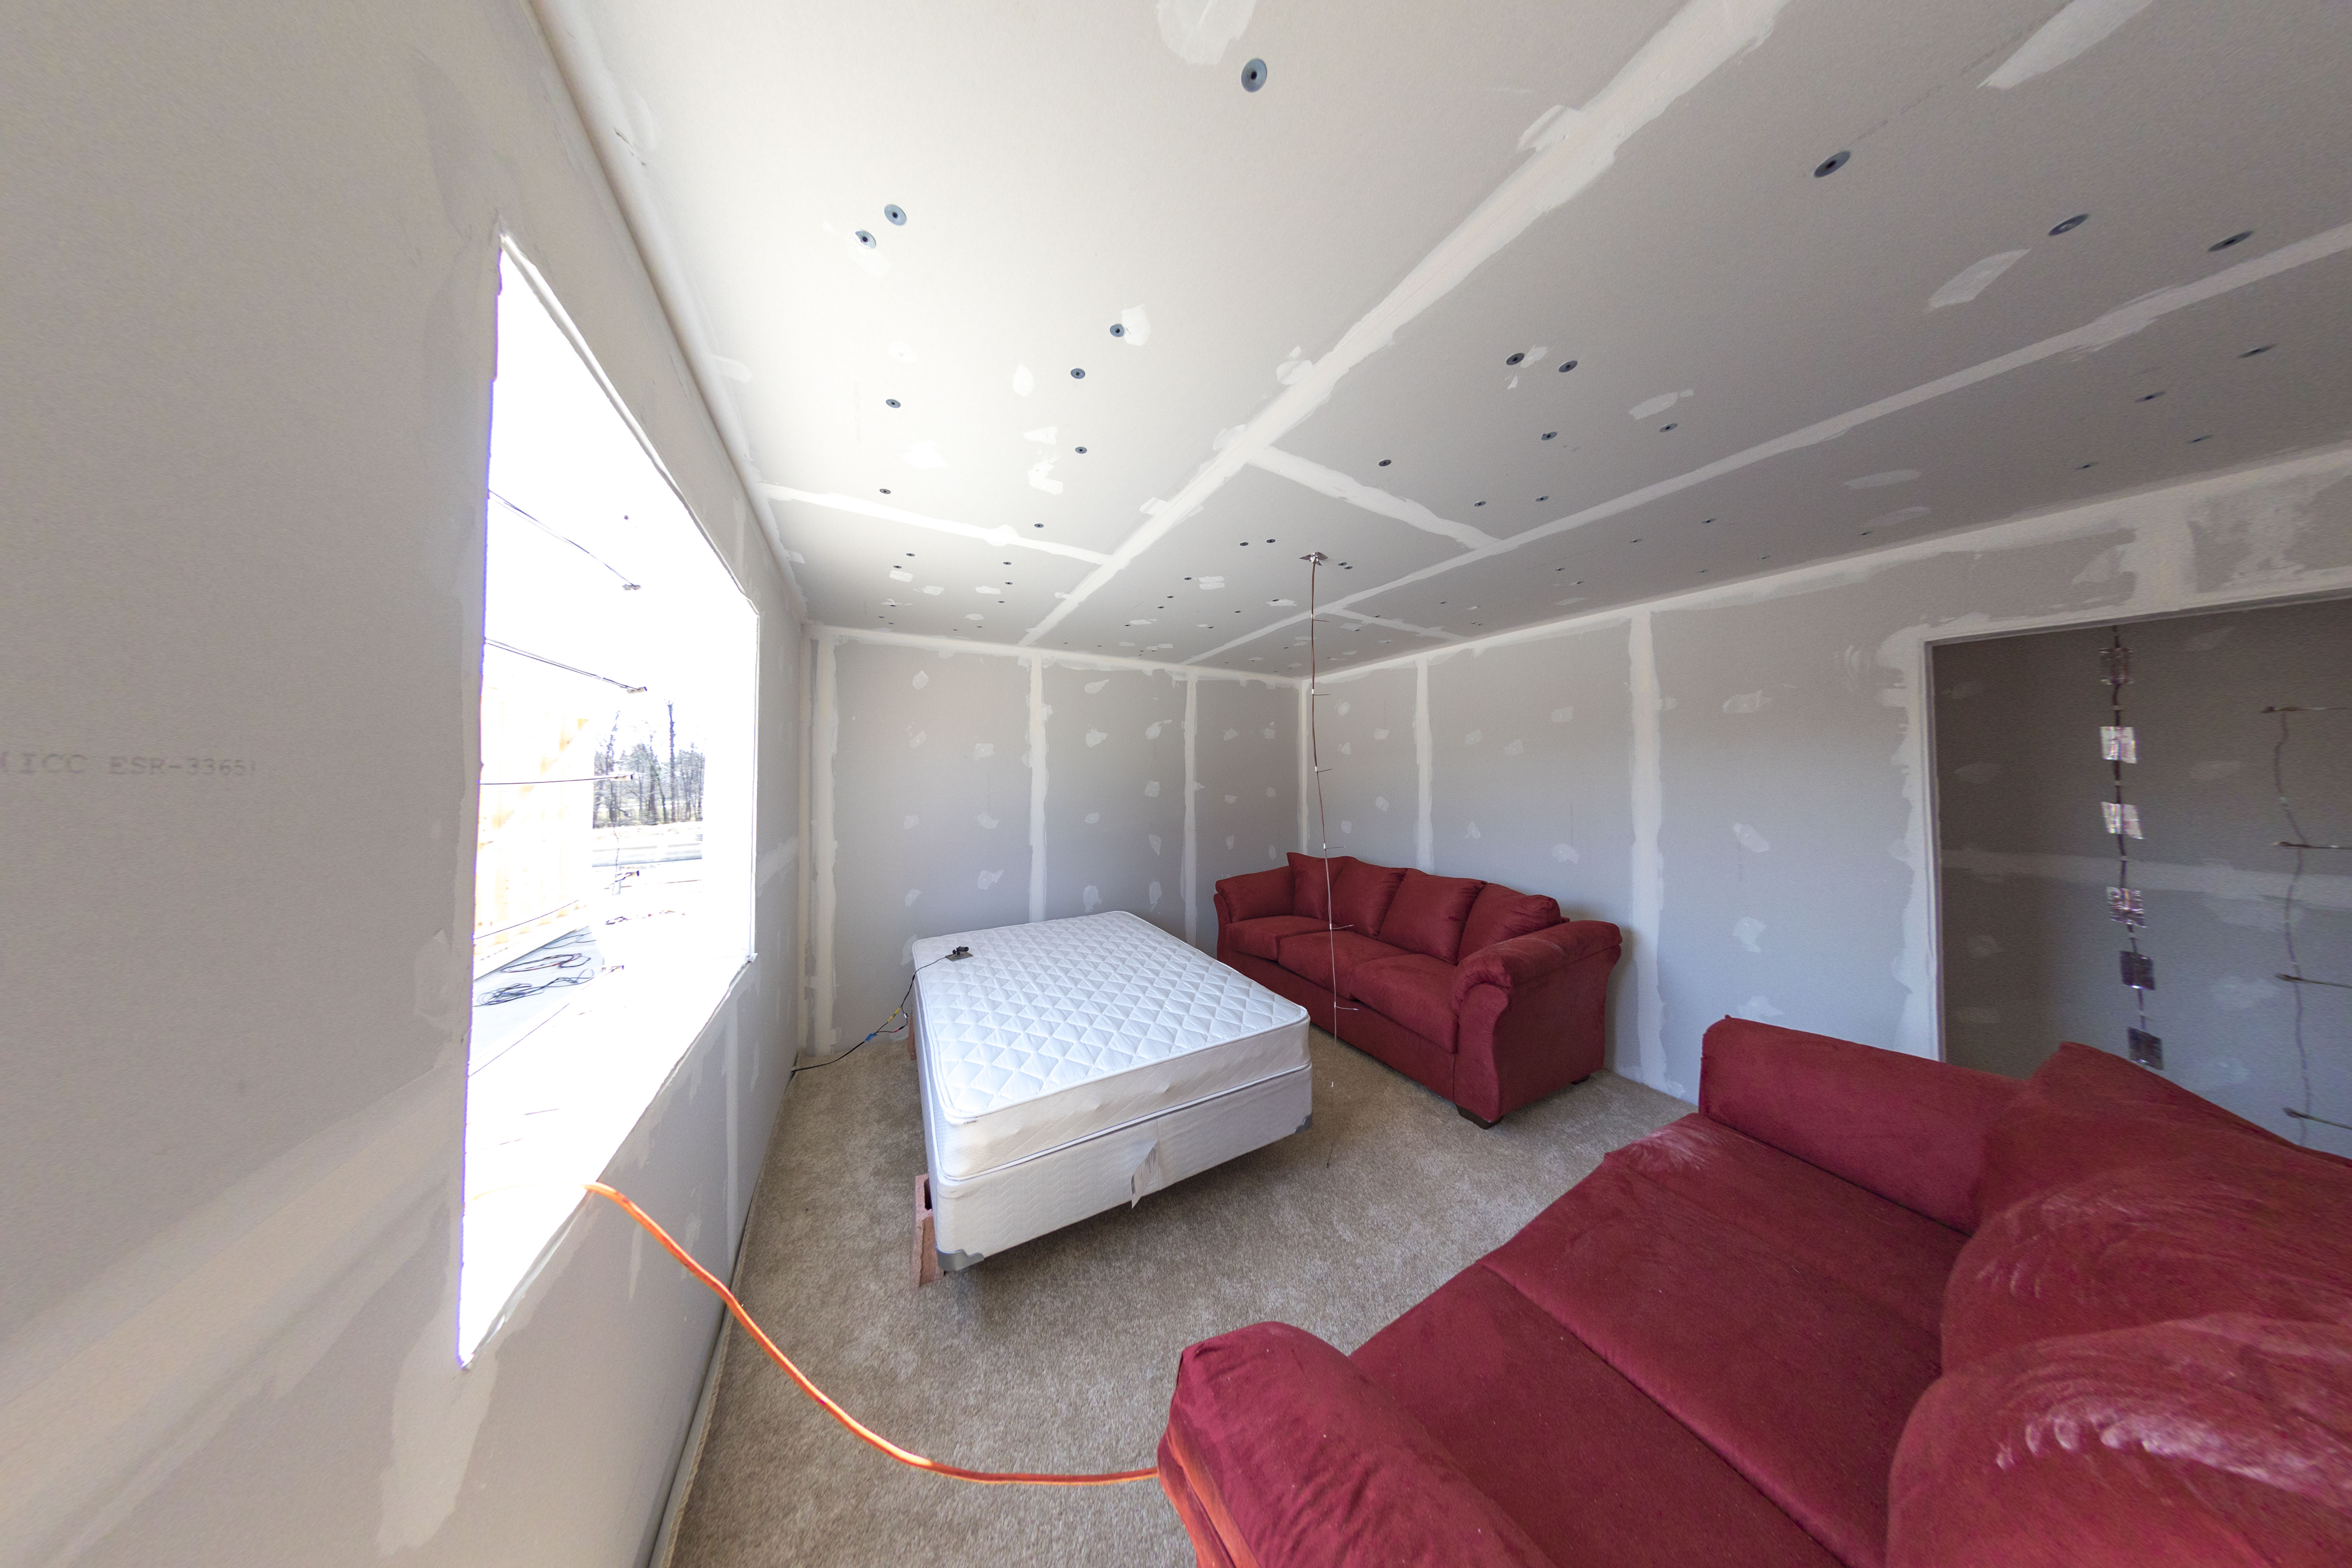
\includegraphics[width=\textwidth]{Figures/Furniture/Exp2to6Furniture.jpg}
	\caption{Experiments 2-6 Furniture Layout}
	\label{fig:Exp2to6Furniture}
\end{figure}

For exact locations of furniture within the structure, see Figure~\ref{fig:Exp1FurnitureDim} and Figure~\ref{fig:Exp2to6FurnitureDim}. 

\begin{figure}[H]
	\centering
	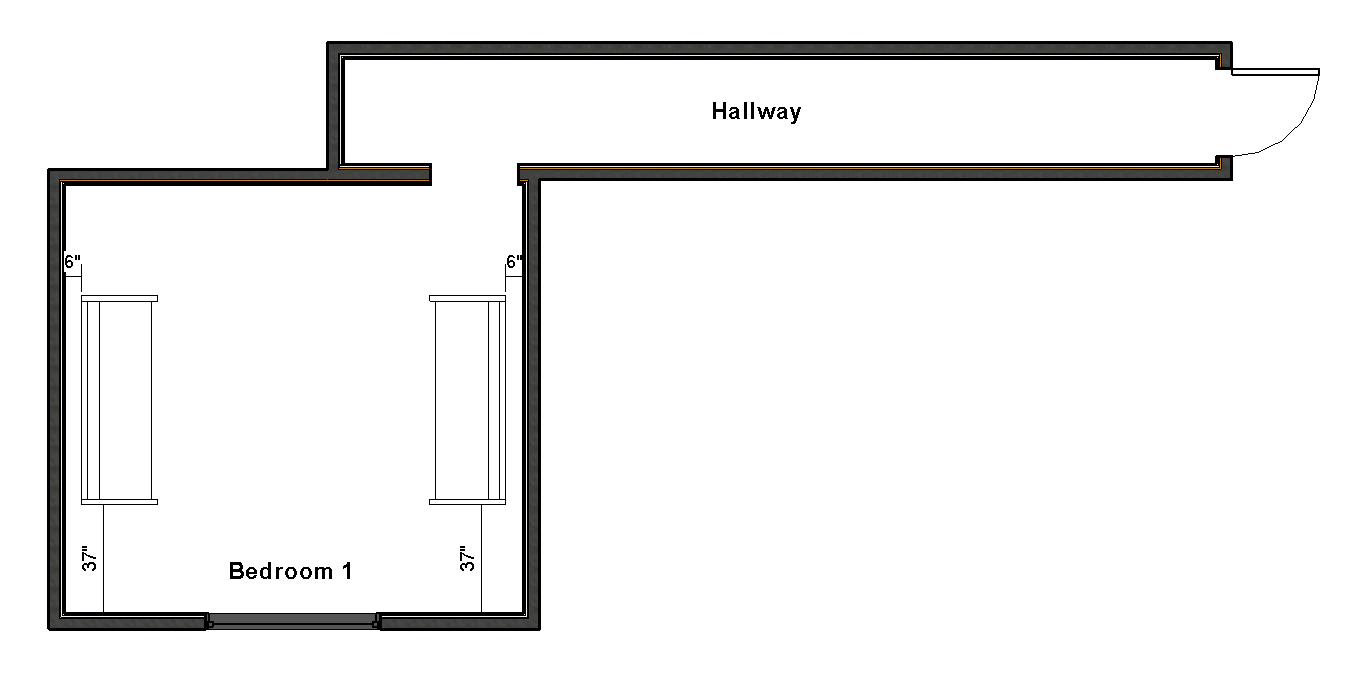
\includegraphics[width=\textwidth]{Figures/Furniture/Exp1FurnitureDimensions.png}
	\caption{Experiment 1 Furniture Layout}
	\label{fig:Exp1FurnitureDim}
\end{figure}

\begin{figure}[H]
	\centering
	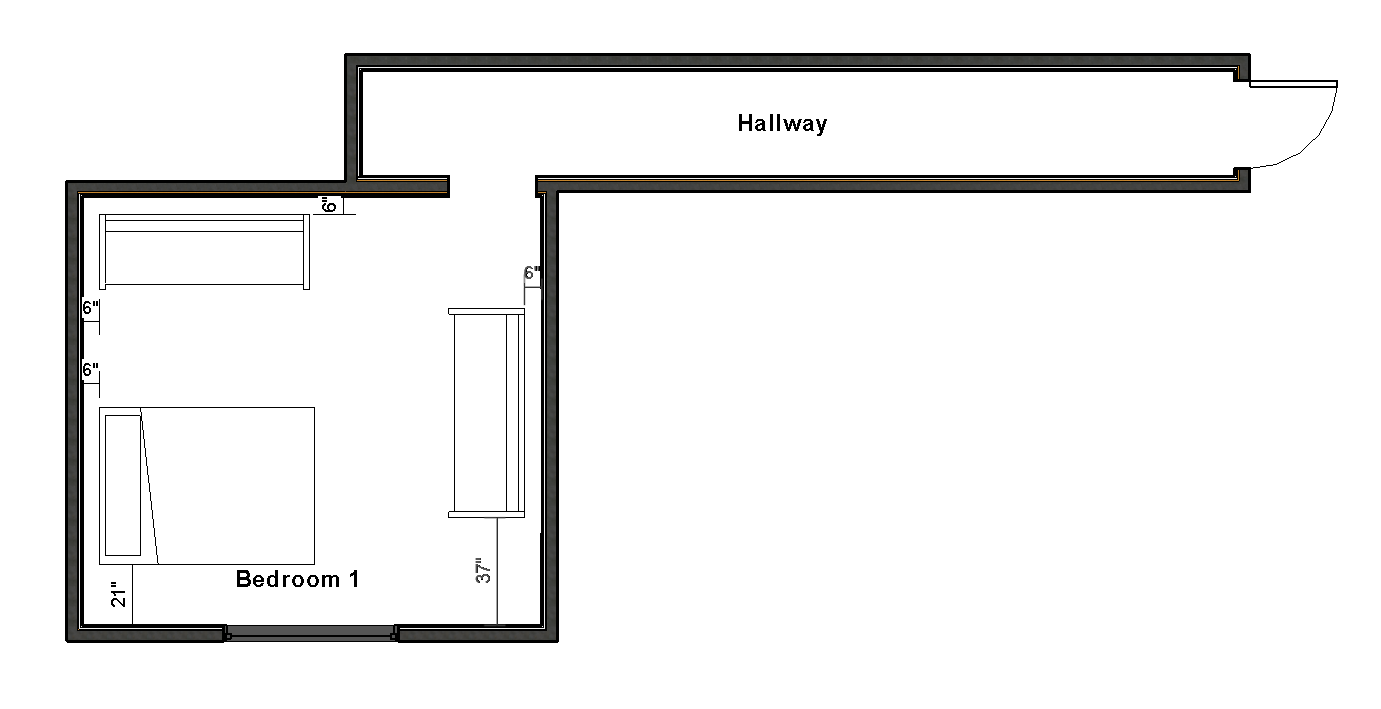
\includegraphics[width=\textwidth]{Figures/Furniture/Exp2to6FurnitureDimensions.png}
	\caption{Experiment 2-6 Furniture Layout}
	\label{fig:Exp2to6FurnitureDim}
\end{figure}

\section{Measurement Locations}

The test fixture was instrumented with temperature, air flow, and pressure sensors. Temperature was measured via Type K thermocouples built into an array. Each array contained 7 measurement locations at 1~ft., 2~ft., 3~ft., 4~ft., 5~ft., 6~ft., and 7~ft. above the floor level. An array was located in the center of the bedroom and in three locations spaced equally along the length of the hallway. Air flow was measured via bi-directional probes. The bedroom 1 doorway (just inside the bedroom and just outside the bedroom) and the entrance of the hallway were instrumented with five bi-directional probes arrayed vertically along the center line at 13.75~in., 27.5~in., 41.25~in., 55~in., and 68.75~in. above the floor. In addition, the bedroom 1 window was instrumented with five bi-directional probes arrayed vertically along the center line at 7~in., 15~in., 23~in., 31~in., and 39~in. above the window sill. Pressure was recorded through a differential pressure transducer in the bedroom as well as the entrance to the hallway at 1~ft., 4~ft., and 7~ft. above the floor. 

The location of each sensor within the structure is shown in Figure~\ref{fig:InstrumentDim}.

\begin{figure}[H]
	\centering
	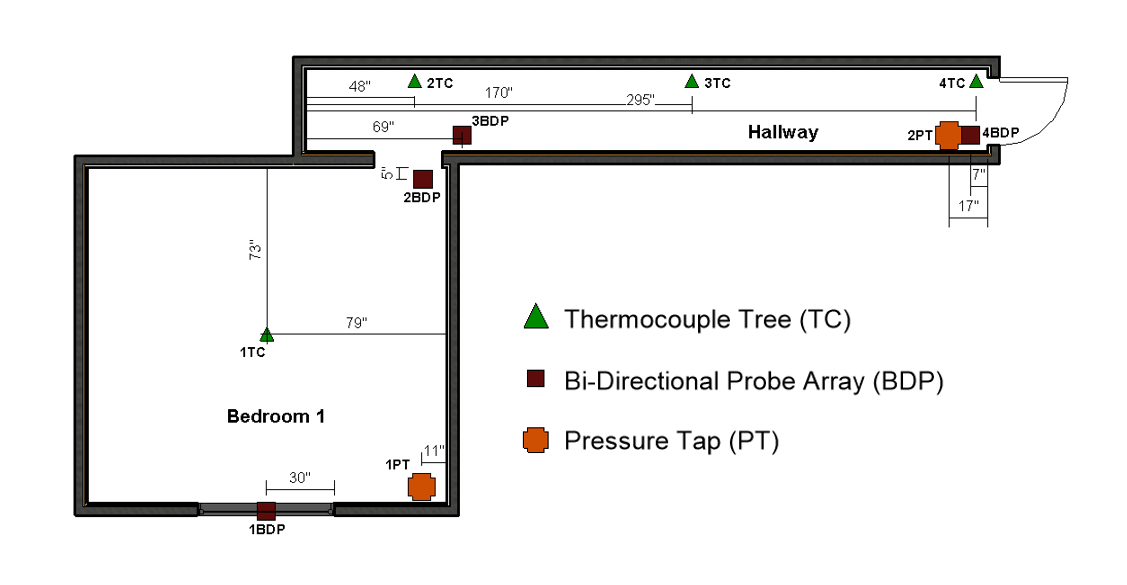
\includegraphics[width=\textwidth]{Figures/Instrumentation/Instrument_Dimensions.png}
	\caption{Instrumentation Layout}
	\label{fig:InstrumentDim}
\end{figure}

\clearpage

\chapter{Test Descriptions}

\paragraph{Experiment 1} \mbox{}

Experiment 1 was a room and contents fire in the bedroom of the structure testing the ability for the fire to regrow after an exterior attack. The door to the hallway and the bedroom window within the structure were open for the duration of the test. The fire was allowed to grow to steady state before suppression. Suppression was conducted from the exterior of the structure via a straight stream on a 150~gpm at 75~psi combination nozzle connected to a 1~3/4~in hoseline. The nozzle firefighter was positioned close to the window opening and the hose stream was directed at the ceiling via a max angle position. Water was applied for approximately 10 seconds. Figure~\ref{fig:Exp1Config} shows the configuration of the structure and Table~\ref{Table:Exp1Interventions} shows at what times interventions were performed. 

% The results of Experiment 1 can be found in Appendix~\ref{App:Exp1Results}. To view the full experiment video \href{https://youtu.be/gl8rc1Nsl1k}{Click Here}.

\begin{figure}[H]
	\centering
	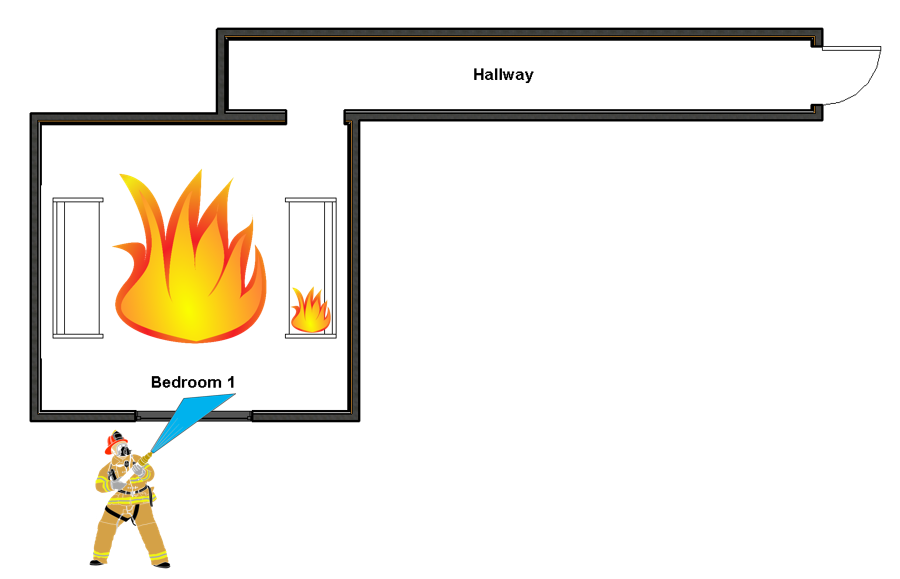
\includegraphics[width=5in]{Howard_Exp_1.png}
	\caption{Experiment 1 Configuration}
	\label{fig:Exp1Config}
\end{figure}

\begin{table}[H]
	\centering
	\caption{Experiment 1 Interventions}
	\begin{tabular}{|c|c|} 
		\hline
		Time & Intervention \\ \hline \hline
		00:00 & Ignition - Bedroom \\ \hline
		04:30 & Exterior Suppression \\ \hline
		13:00 & End Experiment\\ \hline
	\end{tabular}
	\label{Table:Exp1Interventions}
\end{table}

\clearpage

\paragraph{Experiment 2} \mbox{}

Experiment 2 was a room and contents fire in the bedroom of the structure testing the ability for the fire to regrow after an exterior attack. This test was similar to Experiment 1 with the exception of additional fuel loading in the fire room. The details of the differences in the fuel loading can be found in the Fuel Load section above. The door to the hallway and the bedroom window within the structure were open for the duration of the test. The fire was allowed to grow to steady state before suppression. Suppression was conducted from the exterior of the structure via a straight stream on a 150~gpm at 75~psi combination nozzle connected to a 1~3/4~in hoseline. The nozzle firefighter was positioned close to the window opening and the hose stream was directed at the ceiling via a max angle position. Water was applied for approximately 10 seconds. After 16 minutes, it was determined that the fire was not going to re-grow and thus was re-ignited manually in the bedroom and was allowed to grow uninhibited once again until a steady state condition was reached. Exterior suppression was completed as before with water flowing for approximately 8 seconds. After approximately 14 minutes, the fire re-grew to a new steady state and was suppressed one last time using the same method as above with water flowing for approximately 10 seconds. Figure~\ref{fig:Exp2Config} shows the configuration of the structure and Table~\ref{Table:Exp2Interventions} shows at what times interventions were performed.  

% The results of Experiment 1 can be found in Appendix~\ref{App:Exp1Results}. To view the full experiment video \href{https://youtu.be/gl8rc1Nsl1k}{Click Here}.

\begin{figure}[H]
	\centering
	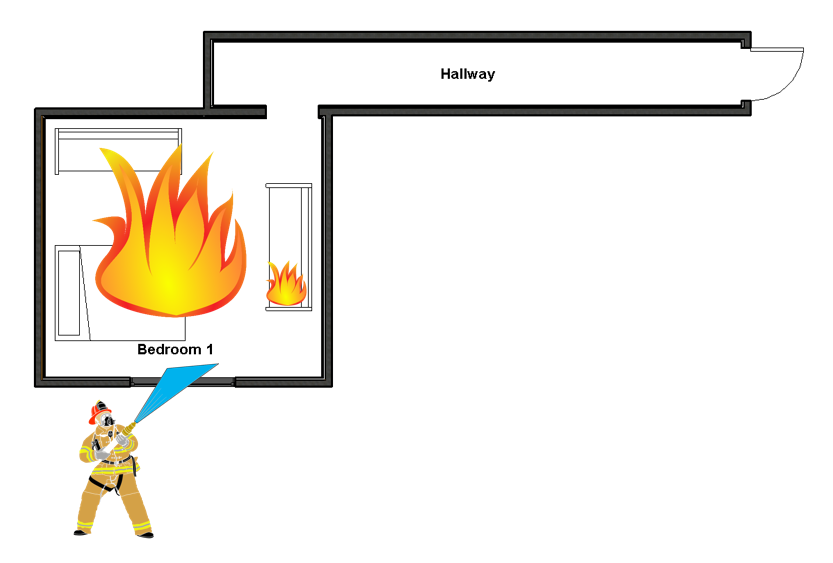
\includegraphics[width=5in]{Howard_Exp_2.png}
	\caption{Experiment 2 Configuration}
	\label{fig:Exp2Config}
\end{figure}

\begin{table}[H]
	\centering
	\caption{Experiment 2 Interventions}
	\begin{tabular}{|c|c|} 
		\hline
		Time & Intervention \\ \hline \hline
		00:00 & Ignition - Bedroom \\ \hline
		05:00 & Exterior Suppression \\ \hline
		21:00 & Second Ignition - Bedroom \\ \hline
		27:00 & Exterior Suppression \\ \hline
		40:20 & Exterior Suppression \\ \hline
		44:00 & End Experiment\\ \hline
	\end{tabular}
	\label{Table:Exp2Interventions}
\end{table}

\clearpage

\paragraph{Experiment 3} \mbox{}

Experiment 3 was a room and contents fire in the bedroom of the structure testing the impact of hose stream air entrainment on fire behavior and suppression capability. The door to the hallway and the bedroom window within the structure were open for the duration of the test. The fire was allowed to grow to steady state before suppression. Suppression was conducted from the interior of the structure via a straight stream on a 150~gpm at 75~psi combination nozzle connected to a 1~3/4~in hoseline. The nozzle firefighter advanced down the hallway and the hose stream was directed ahead in a wall-ceiling-wall pattern before entering the fire room for final extinguishment. Figure~\ref{fig:Exp3Config} shows the configuration of the structure and Table~\ref{Table:Exp3Interventions} shows at what times interventions were performed.  

% The results of Experiment 1 can be found in Appendix~\ref{App:Exp1Results}. To view the full experiment video \href{https://youtu.be/gl8rc1Nsl1k}{Click Here}.

\begin{figure}[H]
	\centering
	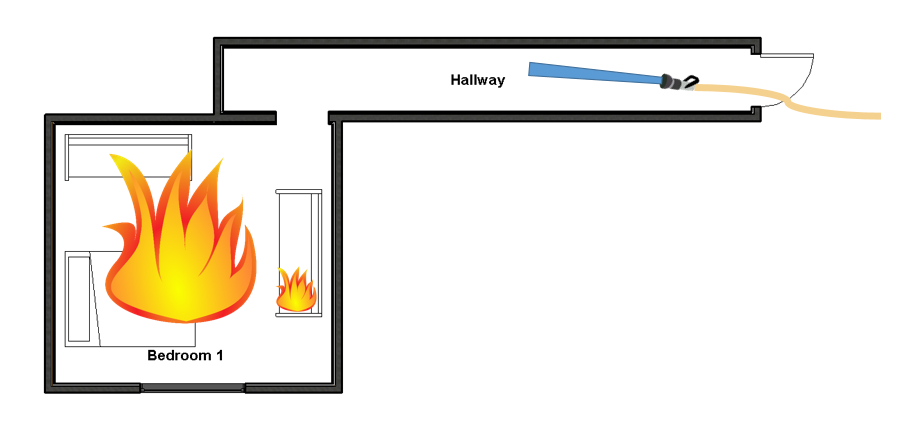
\includegraphics[width=5in]{Howard_Exp_3.png}
	\caption{Experiment 3 Configuration}
	\label{fig:Exp3Config}
\end{figure}

\begin{table}[H]
	\centering
	\caption{Experiment 3 Interventions}
	\begin{tabular}{|c|c|} 
		\hline
		Time & Intervention \\ \hline \hline
		00:00 & Ignition - Bedroom \\ \hline
		05:00 & Interior Suppression \\ \hline
		15:00 & End Experiment\\ \hline
	\end{tabular}
	\label{Table:Exp3Interventions}
\end{table}

\clearpage

\paragraph{Experiment 4} \mbox{}

Experiment 4 was a room and contents fire in the bedroom of the structure testing the impact of hose stream air entrainment on fire behavior and suppression capability. The door to the hallway and the bedroom window within the structure were open for the duration of the test. The fire was allowed to grow to steady state before suppression. Suppression was conducted from the interior of the structure via a narrow fog stream on a 150~gpm at 75~psi combination nozzle connected to a 1~3/4~in hoseline. The nozzle firefighter advanced down the hallway and the hose stream was directed ahead in an `O' pattern before entering the fire room for final extinguishment. Figure~\ref{fig:Exp4Config} shows the configuration of the structure and Table~\ref{Table:Exp4Interventions} shows at what times interventions were performed. 

% The results of Experiment 1 can be found in Appendix~\ref{App:Exp1Results}. To view the full experiment video \href{https://youtu.be/gl8rc1Nsl1k}{Click Here}.

\begin{figure}[H]
	\centering
	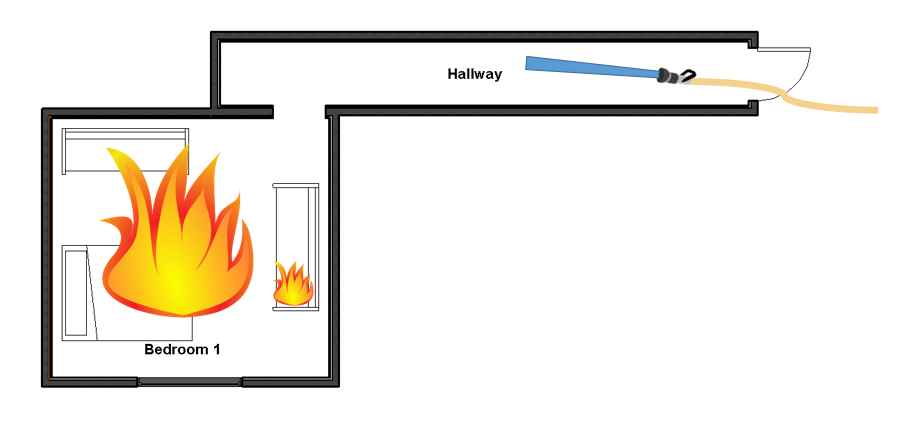
\includegraphics[width=5in]{Howard_Exp_4.png}
	\caption{Experiment 4 Configuration}
	\label{fig:Exp4Config}
\end{figure}

\begin{table}[H]
	\centering
	\caption{Experiment 4 Interventions}
	\begin{tabular}{|c|c|} 
		\hline
		Time & Intervention \\ \hline \hline
		00:00 & Ignition - Bedroom \\ \hline
		07:30 & Interior Suppression \\ \hline
		14:00 & End Experiment\\ \hline
	\end{tabular}
	\label{Table:Exp4Interventions}
\end{table}

\clearpage

\paragraph{Experiment 5} \mbox{}

Experiment 5 was a room and contents fire in the bedroom of the structure testing the impact of door control. The bedroom window within the structure was open for the duration of the test. The fire was allowed to grow to steady state before the hall door was manipulated from the exterior of the structure. Several iterations of door open and door closed were performed before suppression. Suppression was conducted from the exterior of the structure via a straight stream on a 150~gpm at 75~psi combination nozzle connected to a 1~3/4~in hoseline. The nozzle firefighter was positioned close to the window opening and the hose stream was directed at the ceiling via a max angle position. Water was applied for approximately 10 seconds. Figure~\ref{fig:Exp5Config} shows the configuration of the structure and Table~\ref{Table:Exp5Interventions} shows at what times interventions were performed.

% The results of Experiment 1 can be found in Appendix~\ref{App:Exp1Results}. To view the full experiment video \href{https://youtu.be/gl8rc1Nsl1k}{Click Here}.

\begin{figure}[H]
	\centering
	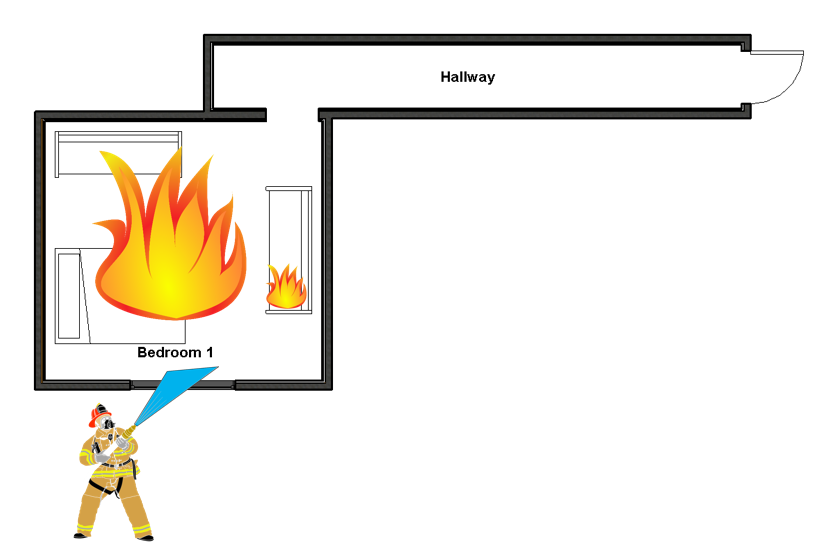
\includegraphics[width=5in]{Howard_Exp_5.png}
	\caption{Experiment 5 Configuration}
	\label{fig:Exp5Config}
\end{figure}

\begin{table}[H]
	\centering
	\caption{Experiment 5 Interventions}
	\begin{tabular}{|c|c|} 
		\hline
		Time & Intervention \\ \hline \hline
		00:00 & Ignition - Bedroom \\ \hline
		04:30 & Hall Door Closed \\ \hline
		05:00 & Hall Door Open \\ \hline
		06:00 & Hall Door Closed \\ \hline
		07:00 & Hall Door Open \\ \hline
		08:00 & Hall Door Closed \\ \hline
		09:00 & Hall Door Open \\ \hline
		11:00 & Exterior Suppression \\ \hline
		20:00 & End Experiment\\ \hline
	\end{tabular}
	\label{Table:Exp5Interventions}
\end{table}

\clearpage

\paragraph{Experiment 6} \mbox{}

Experiment 6 was a room and contents fire in the bedroom of the structure testing the impact of door control. The bedroom window within the structure was closed for the duration of the test. The fire was allowed to grow to steady state before the hall door was manipulated from the exterior of the structure. Several iterations of door open and door closed were performed before the bedroom window was ventilated from the exterior. Additional manipulations of the hall door followed ventilation and before interior suppression was conducted. Suppression was conducted from the interior of the structure via a straight stream on a 150~gpm at 75~psi combination nozzle connected to a 1~3/4~in hoseline. The nozzle firefighter advanced down the hallway and the hose stream was directed ahead in a wall-ceiling-wall pattern before entering the fire room for final extinguishment. Figure~\ref{fig:Exp6Config} shows the configuration of the structure and Table~\ref{Table:Exp6Interventions} shows at what times interventions were performed.

% The results of Experiment 1 can be found in Appendix~\ref{App:Exp1Results}. To view the full experiment video \href{https://youtu.be/gl8rc1Nsl1k}{Click Here}.

\begin{figure}[H]
	\centering
	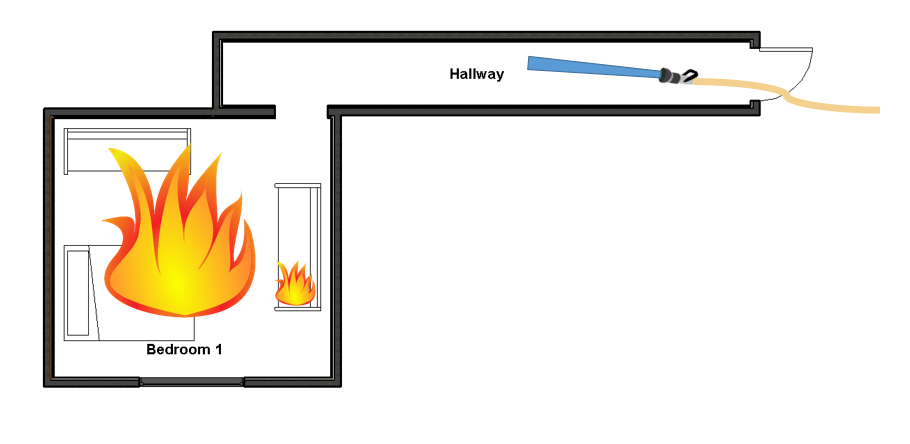
\includegraphics[width=5in]{Howard_Exp_6.png}
	\caption{Experiment 6 Configuration}
	\label{fig:Exp6Config}
\end{figure}

\begin{table}[H]
	\centering
	\caption{Experiment 6 Interventions}
	\begin{tabular}{|c|c|} 
		\hline
		Time & Intervention \\ \hline \hline
		00:00 & Ignition - Bedroom \\ \hline
		04:00 & Hall Door Closed \\ \hline
		04:30 & Hall Door Open \\ \hline
		05:30 & Hall Door Closed \\ \hline
		06:30 & Hall Door Open \\ \hline
		11:30 & Second Ignition - Bedroom \\ \hline
		16:45 & Hall Door Closed \\ \hline
		17:15 & Hall Door Open \\ \hline
		19:45 & Hall Door Closed \\ \hline
		20:15 & Hall Door Open \\ \hline
		21:00 & Bedroom Window Vent \\ \hline
		23:30 & Interior Suppression \\ \hline
		35:00 & End Experiment\\ \hline
	\end{tabular}
	\label{Table:Exp6Interventions}
\end{table}

\clearpage

\end{document}